\section{Trotter Circuits}

To demonstrate the implementability of EDT-style plaquette dynamics on quantum hardware, we retain an archived four-qubit Trotter circuit from the companion workflow. This circuit should be read as an implementation template for plaquette dynamics with local and loop terms, not as the unique gate decomposition of the stripped-down minimal Hamiltonian used in the main-text lambda sweep. Its role is to show that the loop-induced term can be compiled into an explicit circuit structure alongside local control terms.

\begin{figure*}[t]
\centering
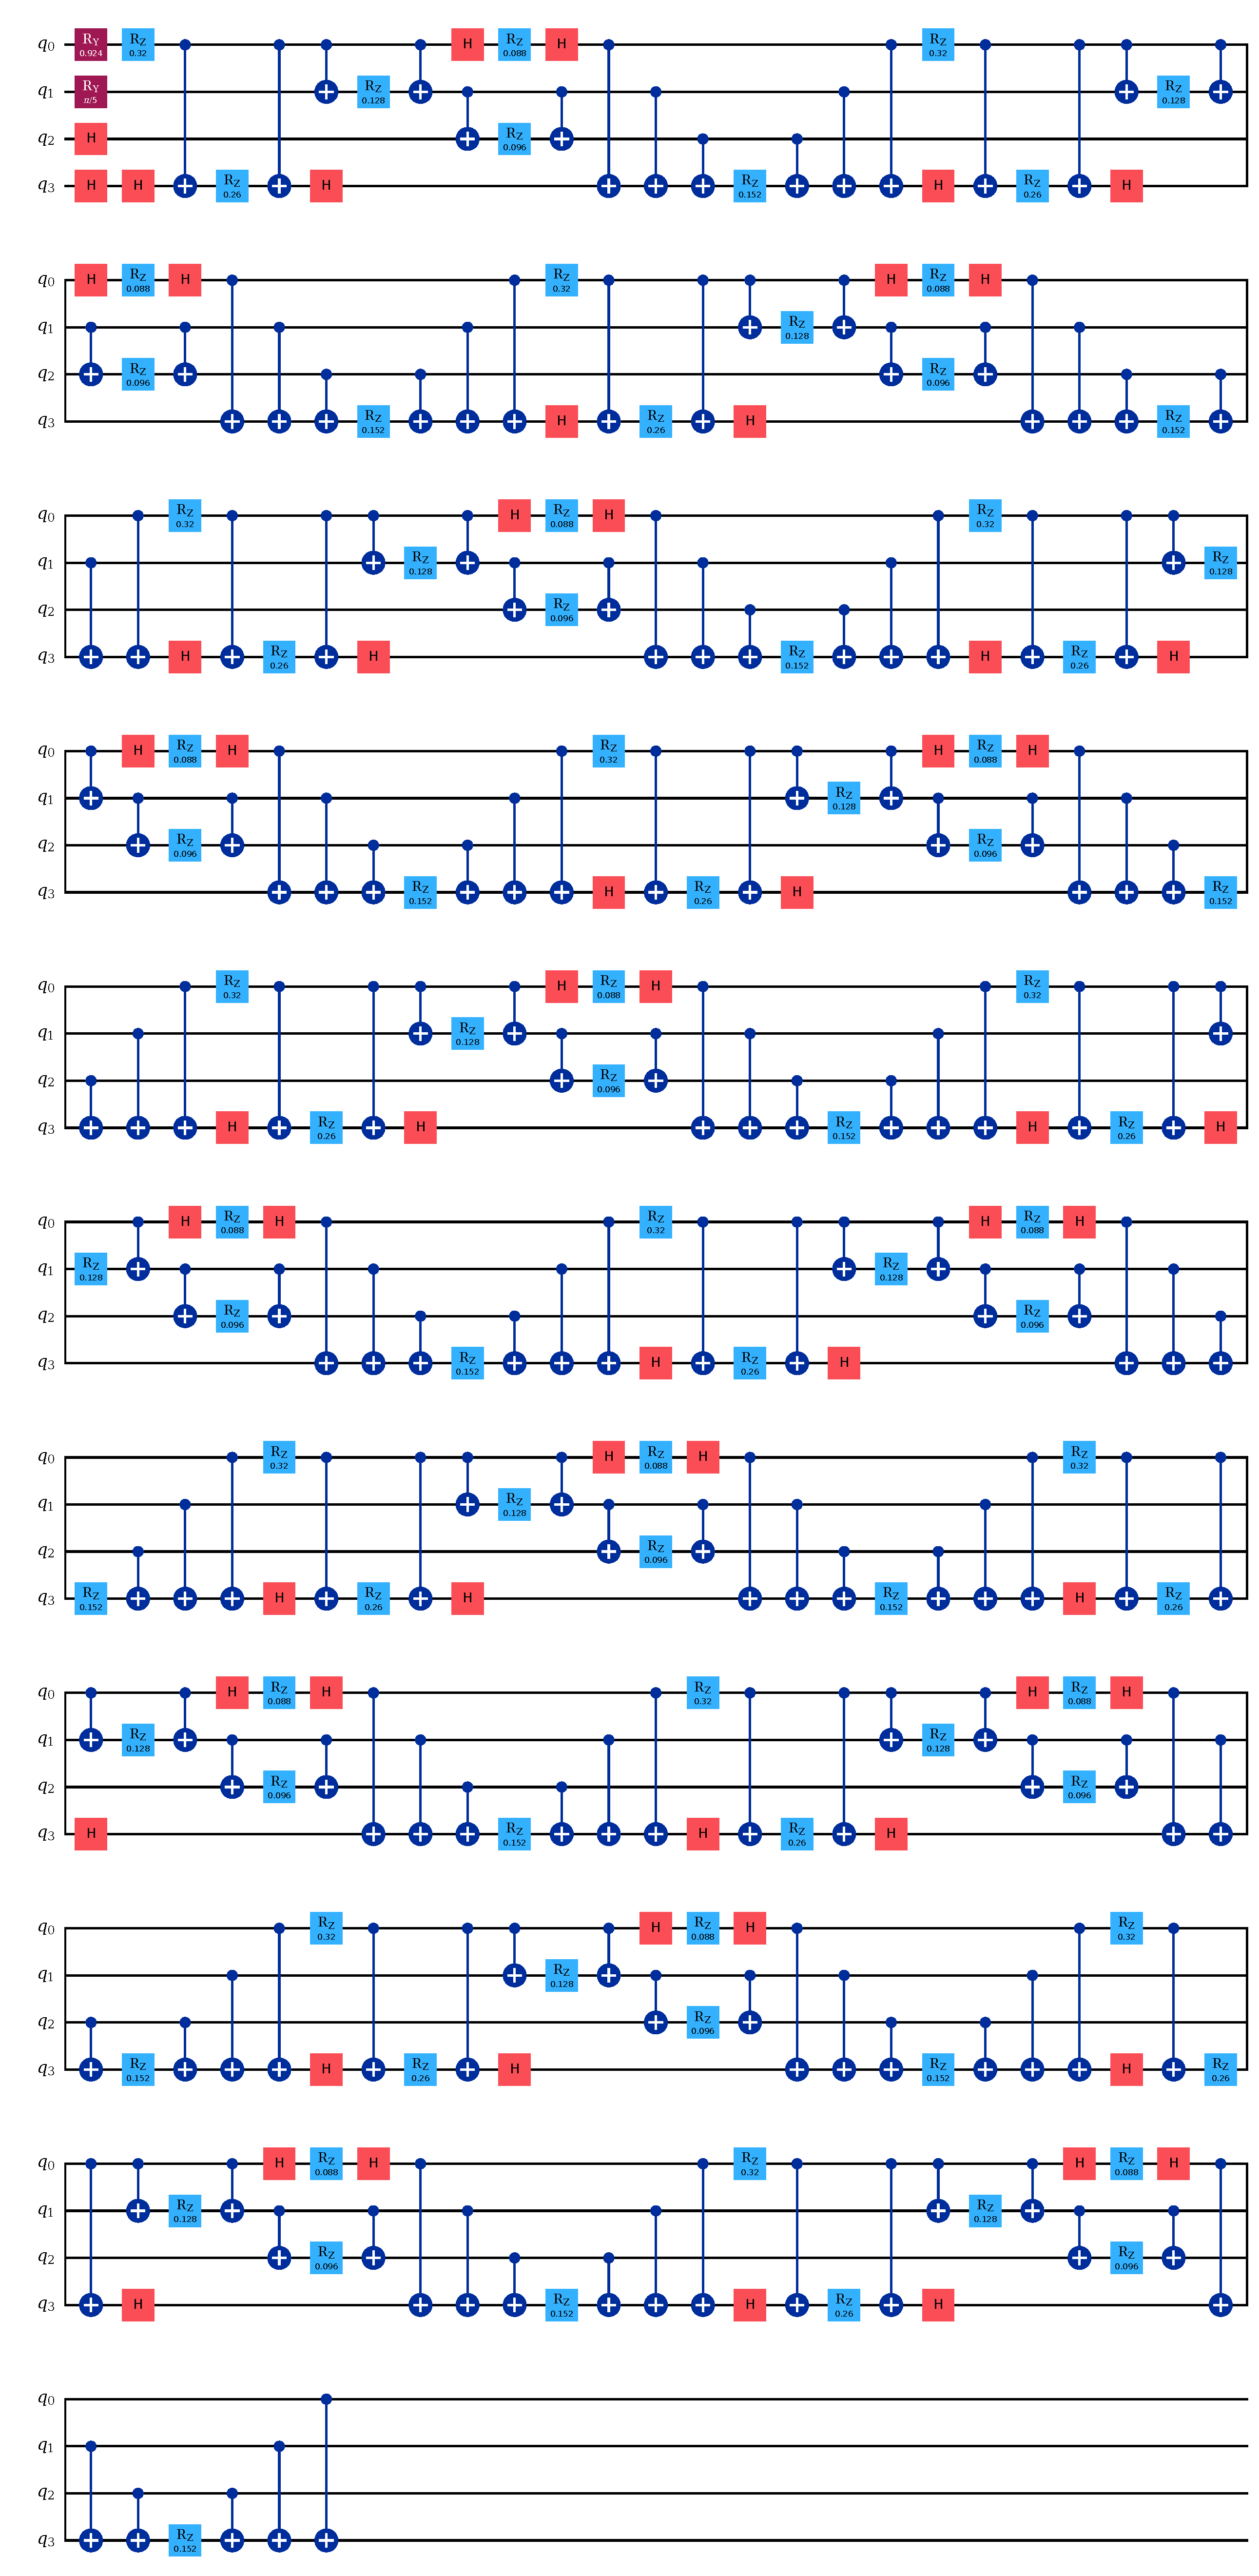
\includegraphics[width=0.52\textwidth]{demo_edt_gyro_trotter_4q_circuit_example.pdf}
\caption{\textbf{S7 | 4-qubit plaquette Trotter realization of EDT dynamics.}
Representative first-order Trotter circuit for an archived plaquette-style four-qubit workflow. The plaquette unitary $e^{-i \lambda Z_0 Z_1 Z_2 Z_3}$ generates multi-qubit entanglement associated with loop topology, while the remaining gates illustrate the inclusion of local control and interaction terms in a gate-based implementation.}
\label{fig:si_4q_plaquette_trotter_circuits}
\end{figure*}
